\documentclass[12pt]{article}
\usepackage[margin=1in]{geometry}
\usepackage{fontspec}
\setmainfont{Arial}
% Soporte para emojis en Windows (ajusta si tienes otra fuente de emojis)
\newfontfamily\emojifont{Segoe UI Emoji}
\usepackage{graphicx}
\usepackage{float}
\usepackage{caption}
\let\oldincludegraphics\includegraphics
\renewcommand{\includegraphics}[2][]{%
  \oldincludegraphics[width=0.5\textwidth,#1]{#2}%
}
\captionsetup{format=plain, labelfont=bf, textfont=normalfont, singlelinecheck=false}
\captionsetup[figure]{skip=10pt}
\usepackage{amsmath,amssymb}

\title{Ejercicios resuelto\\por\\Anselmo Estrada Roa\\Análisis Matemático I\\1er cuatrimestre. 2025}
\date{}
\begin{document}

\maketitle

\section*{{\emojifont 📘}TP2 - Ejercicio 20.a}
En este ejercicio se mezclan varios temas: gráficas de funciones, límites y paridad de funciones. Es lindo y raro, como un perro verde. Pero tiene su encanto, ¿no? Vamos directo al enunciado.

\subsection*{Graficar funciones que verifiquen:}
\begin{enumerate}
  \item $f(x)$ continua en $[-2, 3]$, $f(x) > 0$ en $(-1, 1)$ y discontinua en $x = 3$.
  \item $g(x)$ impar, con una discontinuidad inevitable en $x = 2$, una discontinuidad evitable en $x = 3$ y $\lim_{x \to \infty} g(x) = 5$.
  \item $h(x)$ par, continua y positiva en $[0, 1]$, $\lim_{x \to 1^+} h(x) = -2$, $h(3) = -2$ y con una discontinuidad evitable en $x = 3$.
\end{enumerate}

\section*{Antes de comenzar}
Ojo: van a ser funciones \textbf{a tramos} sí o sí, porque nos están pidiendo discontinuidades inevitables, y esas generalmente aparecen como \textbf{saltos} o \textbf{asíntotas}.

\begin{figure}[H]
  \centering
  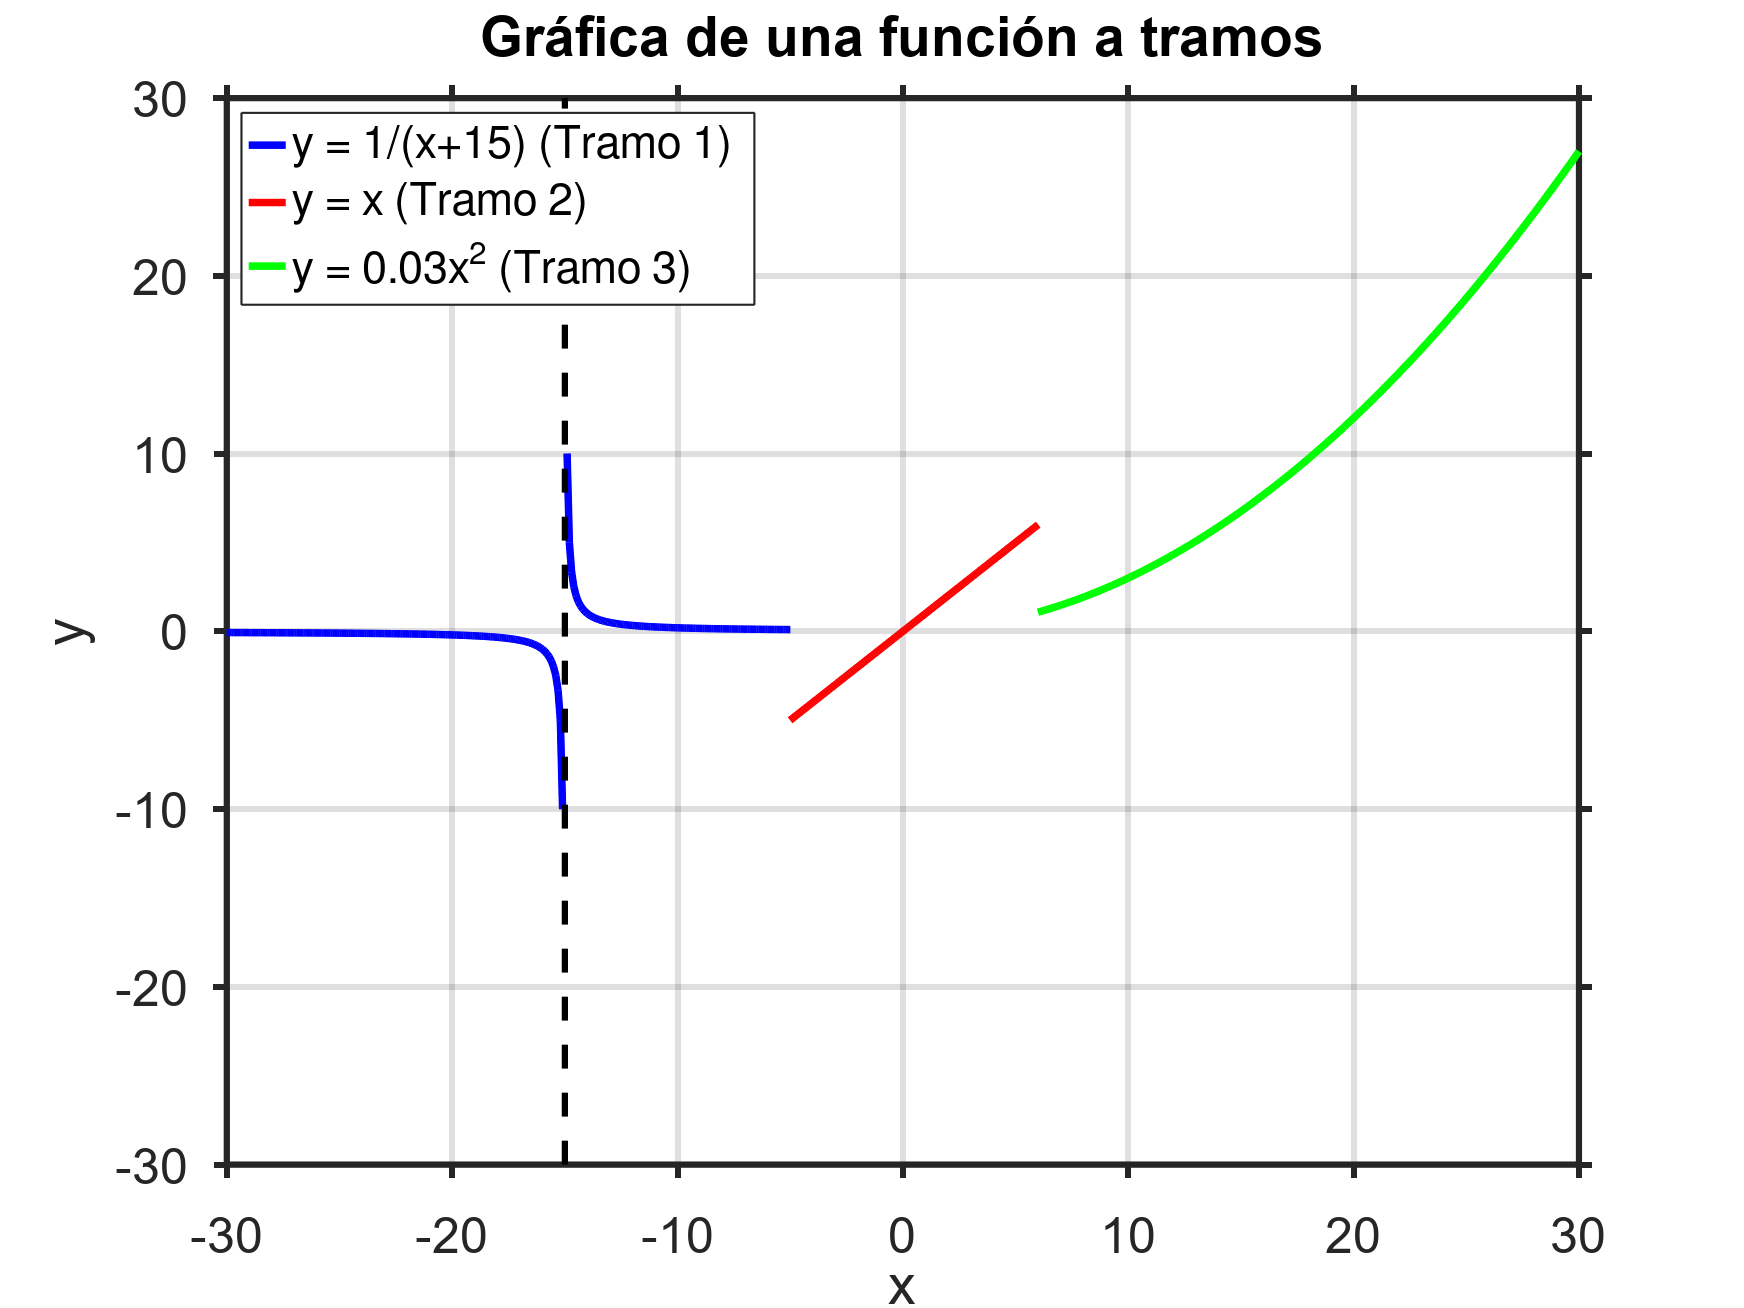
\includegraphics{img/f(x)-a-tramos.png}
  \caption{Gráfico de una función a tramos inventada por mí. Fijate que los tramos en azul son una hipérbola $y = \frac{1}{x+15}$, pero el resto de la función tiene otra definición.}
\end{figure}

Con este pequeño tip... ¡vamos a \textit{laburar, loco}! 

\section*{1. Función $f(x)$}
Queremos que:
\begin{itemize}
  \item Sea continua en $[-2,3]$.
  \item Cumpla que $f(x) > 0$ en $(-1,1)$.
  \item Tenga una discontinuidad en $x=3$.
\end{itemize}

\subsection*{Primer tramo}
Arranquemos asegurando que $f(x) > 0$ en $(-1,1)$.  
Para no complicarnos la vida, podemos dibujar una recta constante: $f(x) = 1$ en ese intervalo.

\begin{figure}[H]
  \centering
  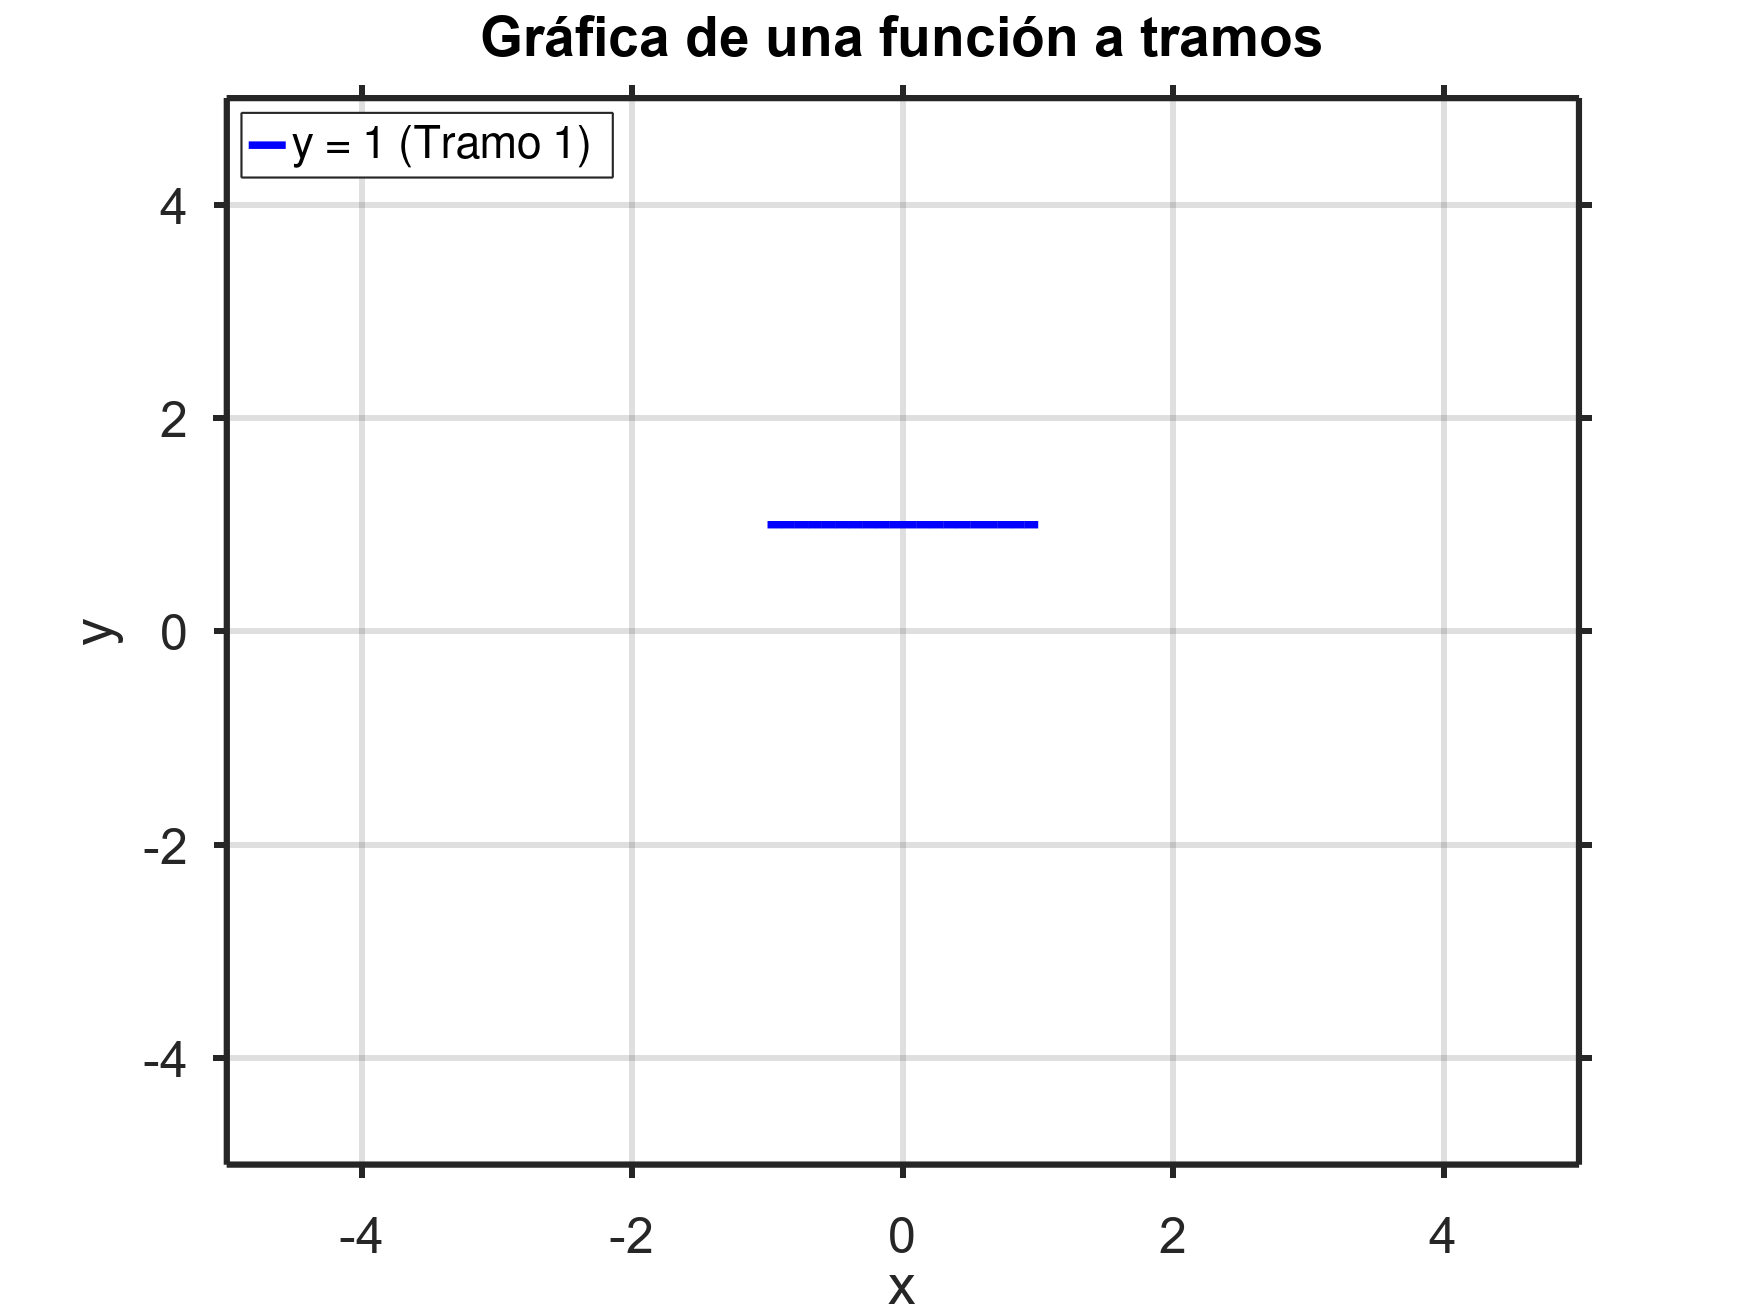
\includegraphics{img/primertramo.png}
  \caption{Empezamos con $y=1$. ¿Por qué tan simple? Porque la vida ya es bastante complicada, pa. Y además, cumple con lo que nos piden.}
\end{figure}

\subsection*{Segundo tramo}
Ahora, agregamos la discontinuidad en $x=3$.  
Una forma sencilla es hacer un salto en la gráfica, por ejemplo bajando a $y=-1$.

\begin{figure}[H]
  \centering
  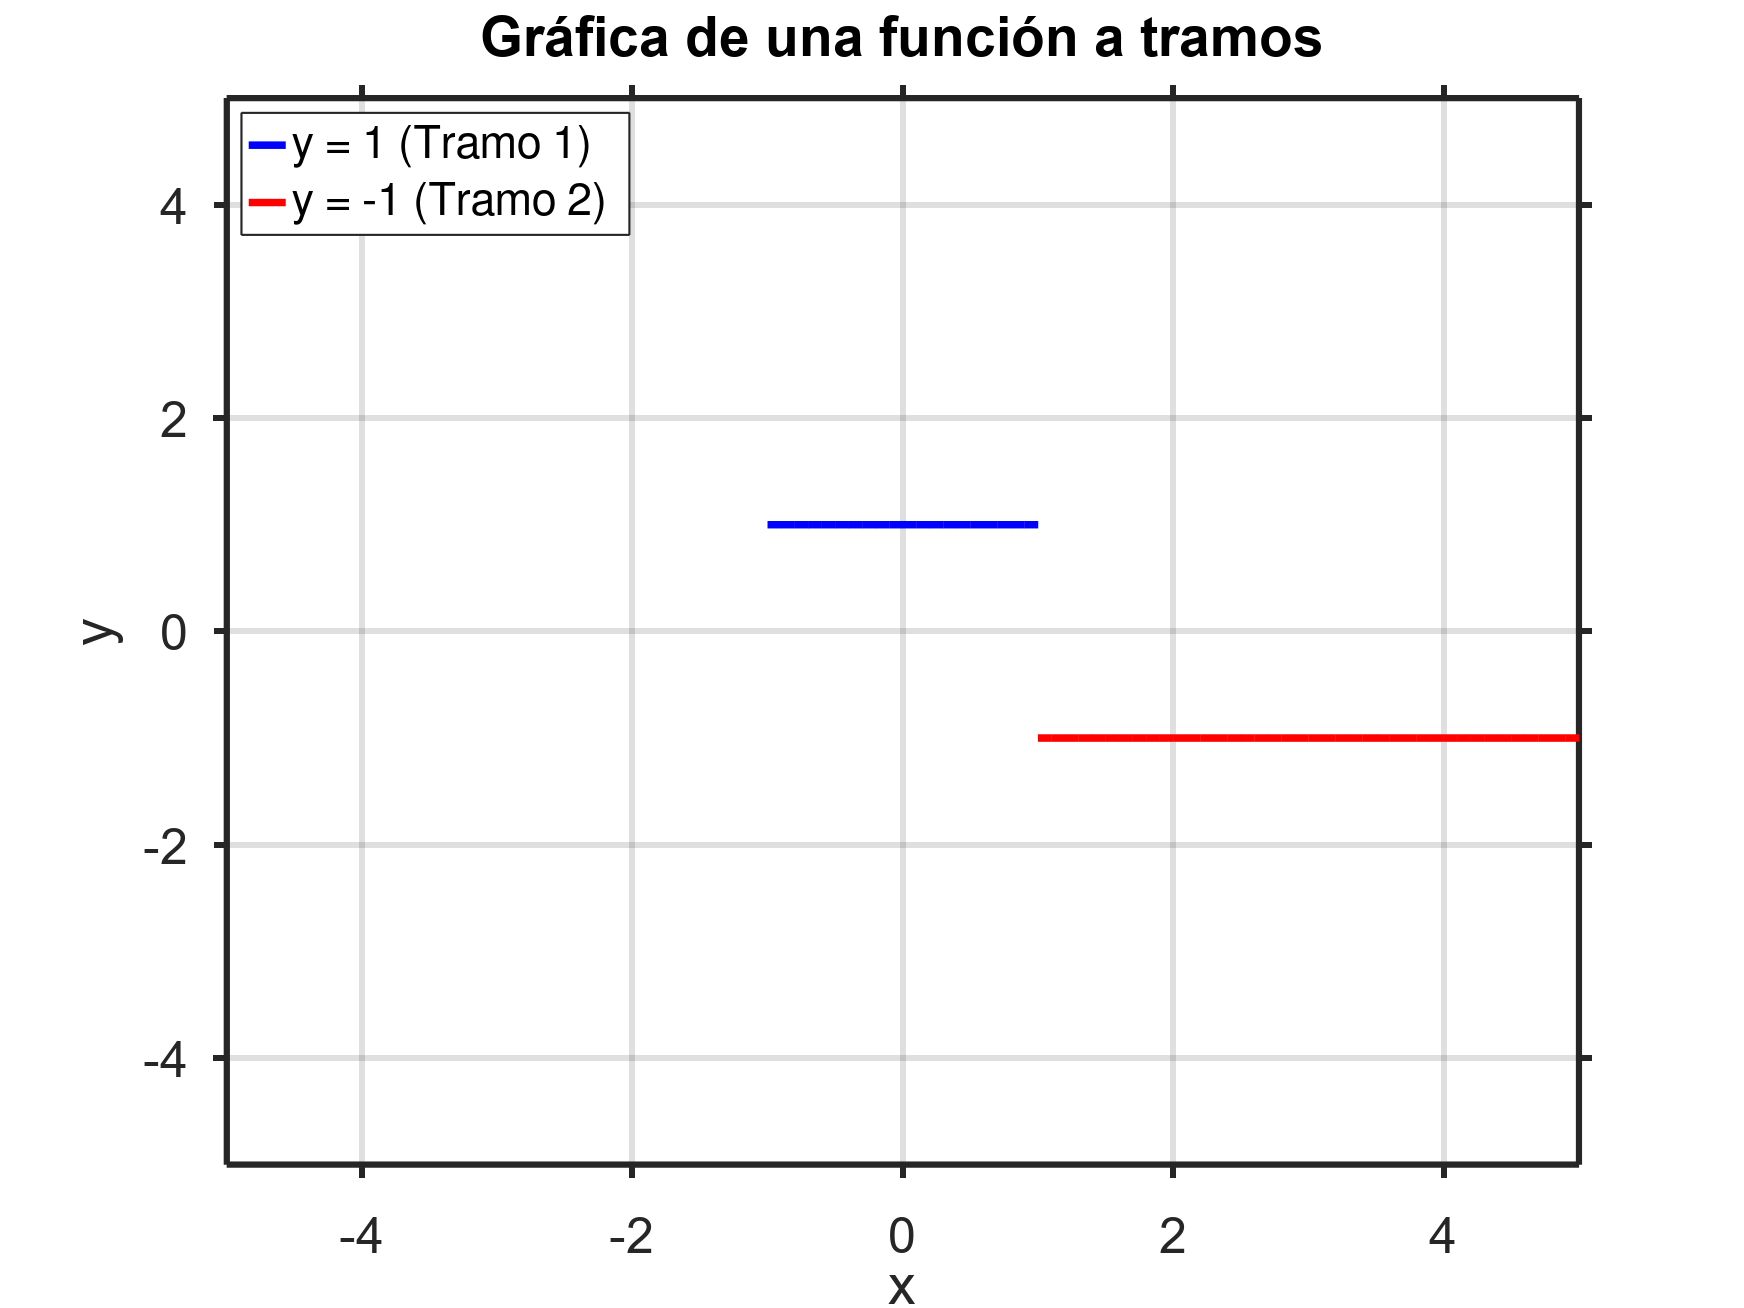
\includegraphics{img/segundotramo.png}
  \caption{Metemos un salto. Ojo: podés elegir otro valor distinto de $-1$ si querés, siempre que no sea $1$, porque ahí no habría discontinuidad real.}
\end{figure}

\subsection*{Tercer tramo}
Finalmente, como debe ser continua en $[-2,3]$ (excepto en $x=3$), extendemos $f(x) = 1$ hacia la izquierda, hasta $x=-2$.

\begin{figure}[H]
  \centering
  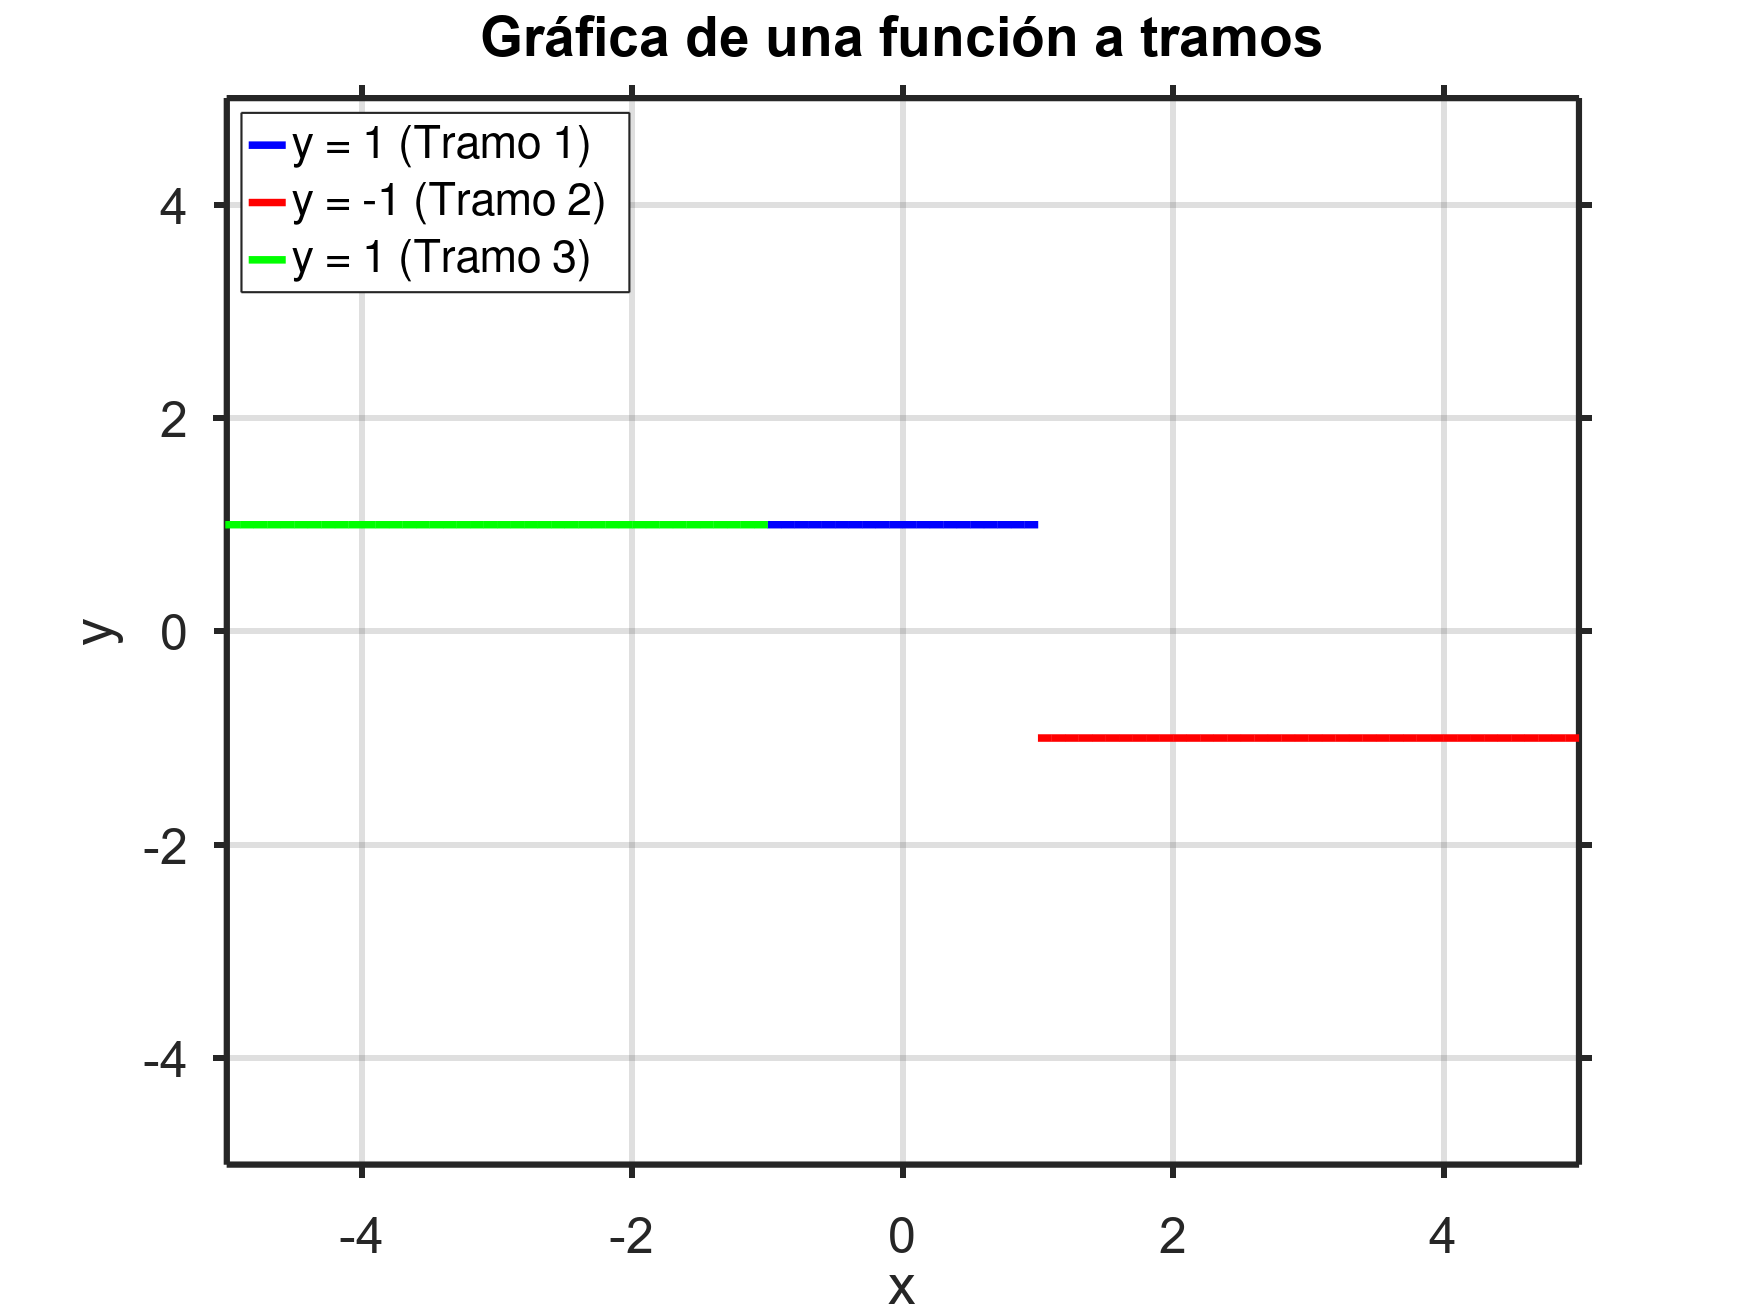
\includegraphics{img/tercertramo.png}
  \caption{Gráfico de la función con el tercer tramo.}
\end{figure}

¿Es esta la única solución? \textbf{No}.  
Podés inventar mil versiones distintas mientras respeten las condiciones. Por ejemplo:

\begin{figure}[H]
  \centering
  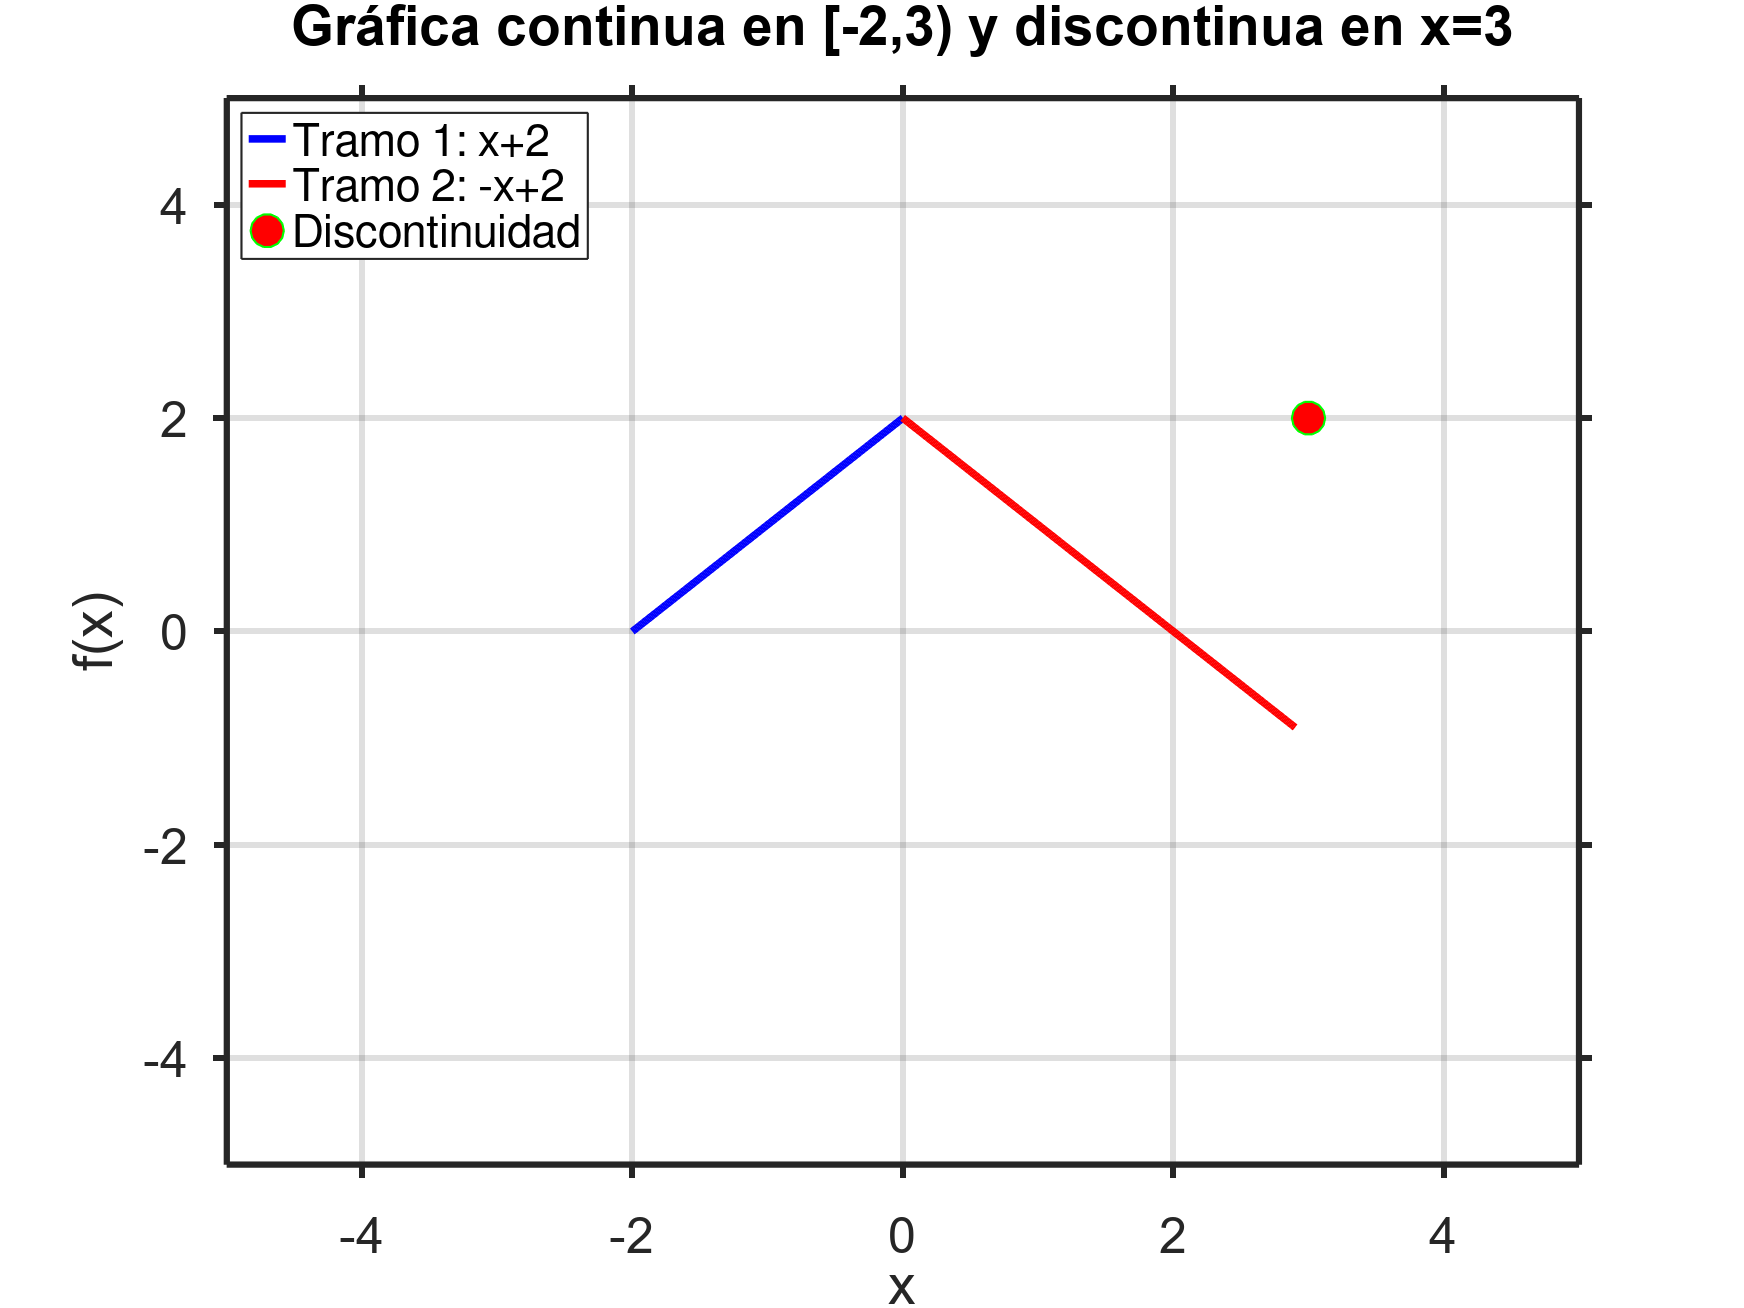
\includegraphics{img/ej001otro-ejemplo.png}
  \caption{Gráfico de la función con otro ejemplo.}
\end{figure}

\section*{2. Función $g(x)$}
Ahora nos toca una función que debe ser:
\begin{itemize}
  \item Impar.
  \item Con una discontinuidad inevitable en $x=2$.
  \item Una discontinuidad evitable en $x=3$.
  \item Y que cumpla $\lim_{x \to \infty} g(x) = 5$.
\end{itemize}
Al ser impar, trabajamos primero para $x>0$ y después reflejamos para $x<0$.

\subsection*{Parte positiva}
Para la discontinuidad evitable en $x=3$, basta con que el valor de $g(3)$ no coincida con el límite lateral.

Para el límite en infinito, pensamos en una función que tienda a 5, como:

\[
  g(x) = 5 + \frac{1}{x-2}
\]

Esta función, además, tiene una asíntota vertical en $x=2$, perfecta para la discontinuidad inevitable que nos piden.

- En $x \in (2,3)$ y $x>3$, usamos esa hipérbola desplazada.

- En $x \in (0,2)$, para algo fácil, podemos usar la recta $y=x$.

\subsection*{Parte negativa}
Ahora reflejamos todo para que sea impar:

- La recta $y=x$ ya es impar, así que no hay problema.

- La hipérbola debe reflejarse también, pasando de $5+\frac{1}{x-2}$ a $-5+\frac{1}{x+2}$.

- Los puntos aislados también se reflejan respetando $g(-x) = -g(x)$.


Así nos queda:

\begin{equation}
  g(x) = 
  \begin{cases}
    -5 + \frac{1}{x+2}, & x \in (-\infty, -3) \cup (-3, -2) \\
    -2, & x = -3 \\
    x, & x \in [-2,2] \\
    2, & x = 3 \\
    5 + \frac{1}{x-2}, & x \in (2,3) \cup (3,\infty)
  \end{cases}
\end{equation}

\begin{figure}[H]
  \centering
  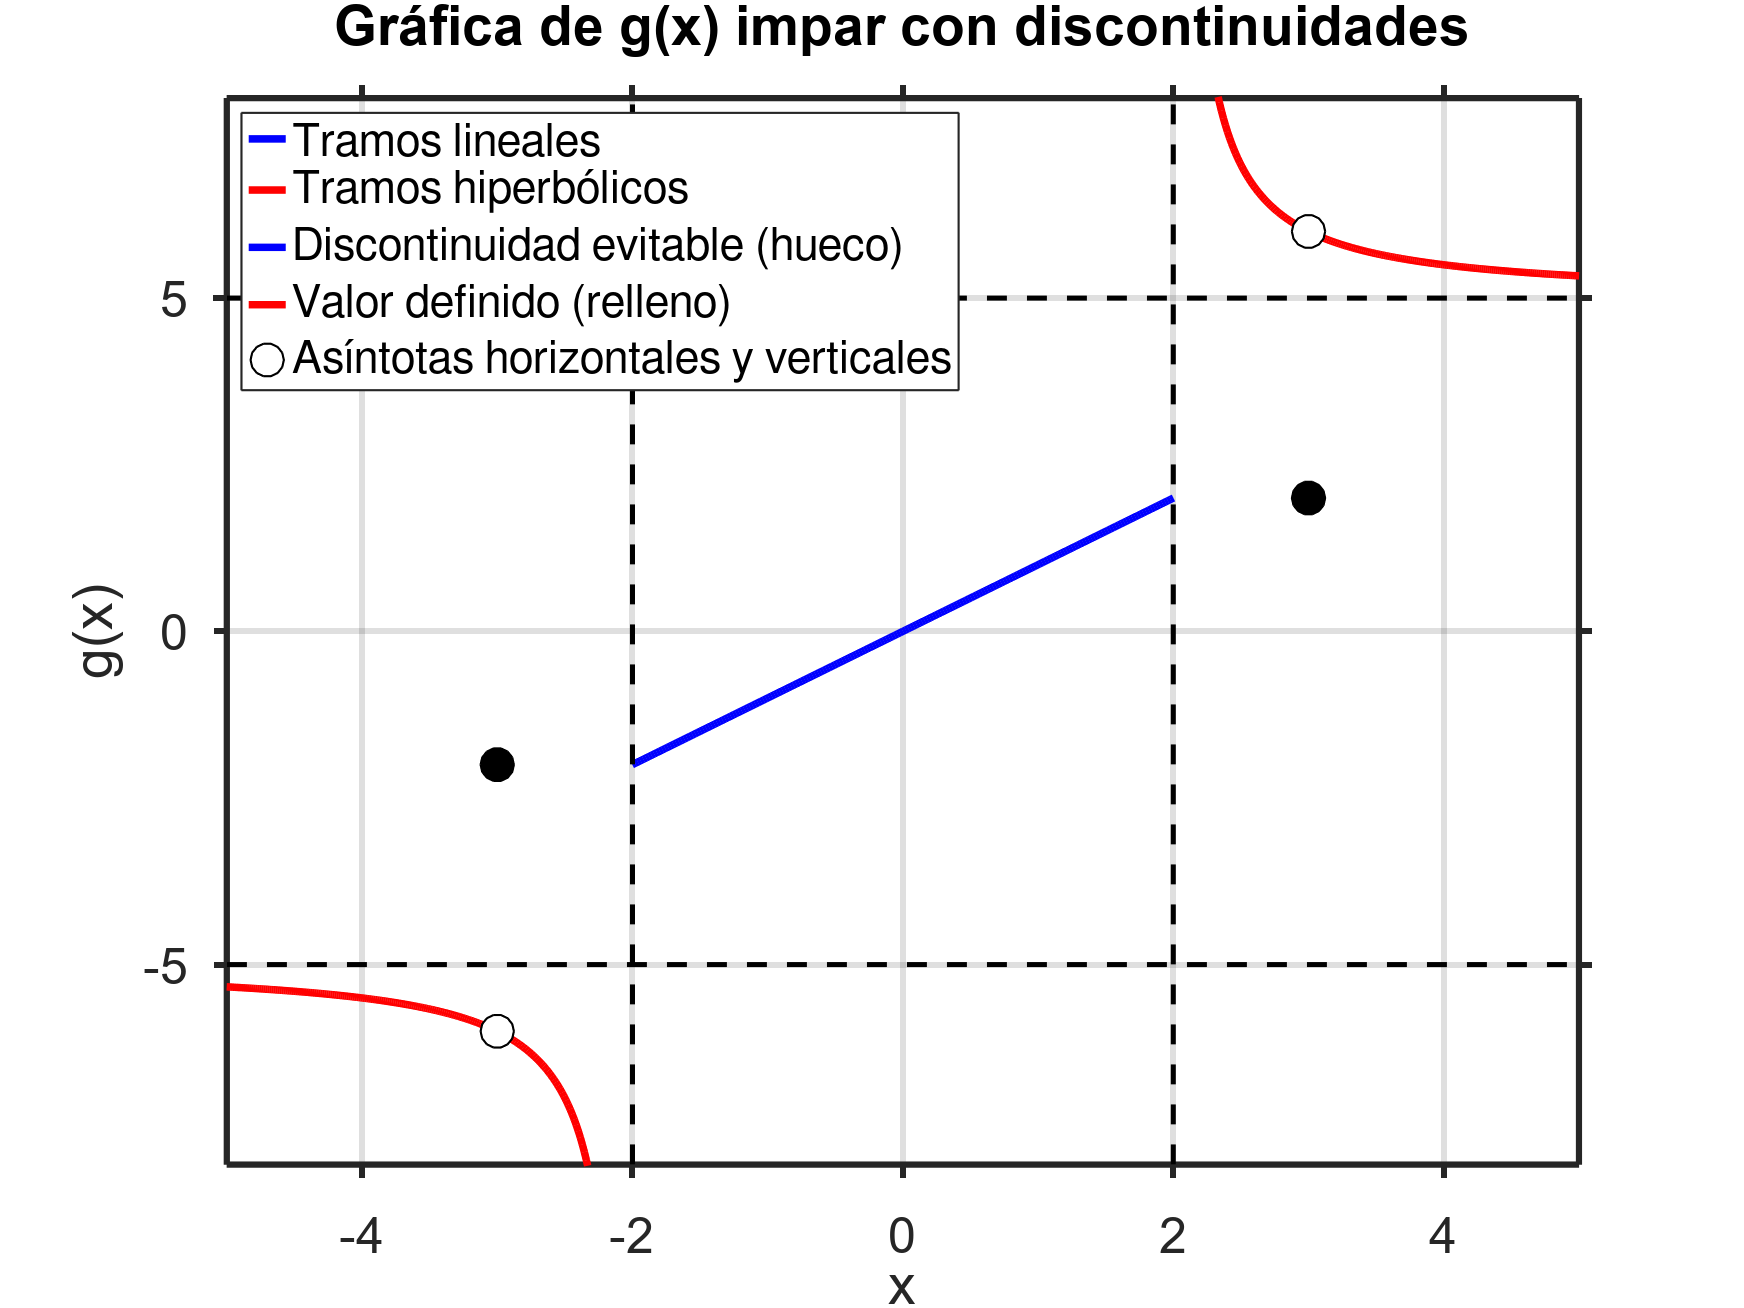
\includegraphics{img/g(x).png}
  \caption{Gráfico de $g(x)$.}
\end{figure}

\section*{3. Función $h(x)$}
Finalmente tenemos una función que debe ser:
\begin{itemize}
  \item Par.
  \item Continua y positiva en $[0,1]$.
  \item Con $\lim_{x \to 1^+} h(x) = -2$.
  \item Que cumpla $h(3) = -2$.
  \item Y con una discontinuidad evitable en $x=3$.
\end{itemize}

Una buena idea sería definir:
- En $[-1,1]$, usamos $h(x) = |x|$ (positivo y par).
- En $(1,2)$ y $(2,3)$, rectas que conecten razonablemente.
- En $x=3$, forzamos $h(3) = -2$, pero no coincidiendo con el límite lateral.

Y para respetar la paridad, reflejamos todo hacia la izquierda.

Una propuesta concreta sería:

\begin{equation}
  h(x) = 
  \begin{cases}
    -x-3, & x \in (-\infty, -3) \cup (-3, -1) \\
    -2, & x = -3 \\
    |x|, & x \in [-1,1] \\
    -2, & x = 3 \\
    x-3, & x \in (1,3) \cup (3,\infty)
  \end{cases}
\end{equation}

\begin{figure}[H]
  \centering
  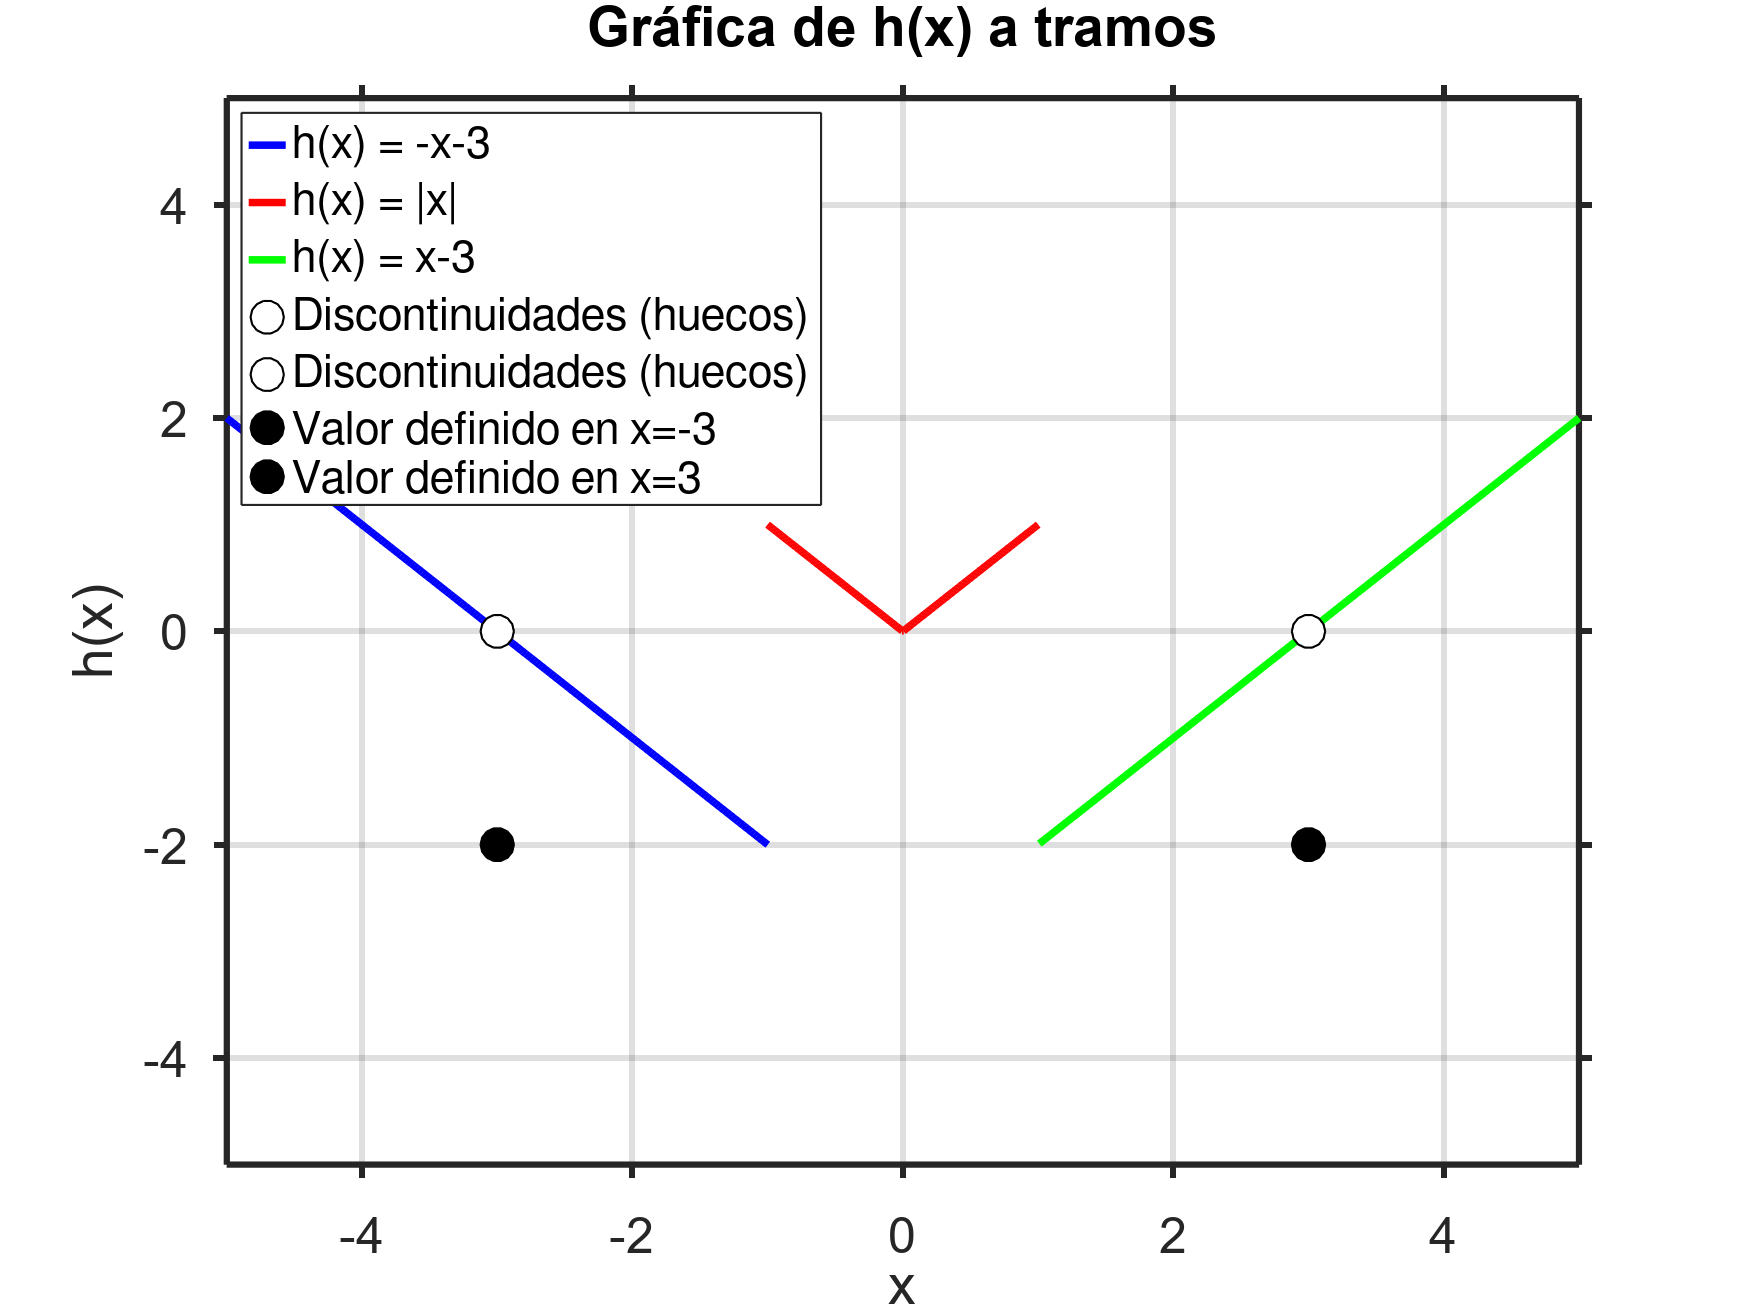
\includegraphics{img/h(x).png}
  \caption{Gráfico de $h(x)$.}
\end{figure}

\section*{{\emojifont 🎯} Conclusión}
Este ejercicio combina muchos conceptos: continuidad, límites, paridad, funciones a tramos, y un poco de creatividad.  
Recordá: \textbf{hay muchas soluciones posibles}, lo importante es respetar las condiciones que nos piden.

\end{document}